\documentclass[landscape,paperwidth=48in,paperheight=36in,fontscale=0.29]{baposter}

\usepackage[T1]{fontenc}
\usepackage[scaled]{helvet}
\usepackage{graphicx}
\usepackage{amsmath}
\usepackage{enumitem}
\usepackage{microtype}
\usepackage{xcolor}
\usepackage{url}

\renewcommand{\familydefault}{\sfdefault}
\urlstyle{same}
\graphicspath{{../paper/figs/}}
\emergencystretch=2em

\setlist[itemize]{leftmargin=*,itemsep=0.34em,topsep=0.18em}
\setlist[enumerate]{leftmargin=1.35em,itemsep=0.32em,topsep=0.15em}

\definecolor{ink}{HTML}{16324F}
\definecolor{accent}{HTML}{0F6C7B}
\definecolor{accentlight}{HTML}{E7F6F8}
\definecolor{sand}{HTML}{F7F4EE}
\definecolor{border}{HTML}{8AA4B6}
\definecolor{muted}{HTML}{5E6A75}
\definecolor{sky}{HTML}{EDF6FA}

\newcommand{\AUROC}{\textsc{AUROC}}
\newcommand{\OOD}{\textsc{OOD}}
\newcommand{\best}[1]{{\sffamily\bfseries #1}}
\newcommand{\statvalue}[1]{{\sffamily\bfseries\fontsize{27}{29}\selectfont #1}}
\newcommand{\statcard}[2]{%
\fcolorbox{border}{sky}{%
\begin{minipage}[c][4.7em][c]{0.47\linewidth}
\centering
\statvalue{#1}\\[-0.12em]
{\sffamily\small #2}
\end{minipage}}}
\newcommand{\resultcallout}[1]{%
\begin{center}
\fcolorbox{border}{accentlight}{%
\parbox{0.92\linewidth}{%
\centering
\sffamily\bfseries\large\color{ink}#1}}
\end{center}}
\newcommand{\footerpanel}[2]{%
\fcolorbox{border}{accentlight}{%
\begin{minipage}[t][4.8em][t]{0.305\linewidth}
{\sffamily\bfseries\large\color{ink}#1}\\[0.35em]
#2
\end{minipage}}}

\begin{document}

\begin{poster}{
 grid=false,
 eyecatcher=false,
 columns=4,
 colspacing=0.85em,
 headerColorOne=ink,
 headerColorTwo=accent,
 borderColor=border,
 boxColorOne=white,
 boxColorTwo=sand,
 headerFontColor=white,
 textborder=faded,
 headerborder=open,
 headershape=roundedright,
 headershade=plain,
 boxshade=plain,
 background=plain,
 bgColorOne=white,
 bgColorTwo=white,
 headerheight=0.115\textheight,
 boxpadding=0.7em,
 linewidth=1.6pt,
 headerfont=\sffamily\bfseries\Large,
 textfont={\small}
}
{}
{
\begin{minipage}{0.99\linewidth}
\centering
{\sffamily\bfseries\fontsize{18}{20}\selectfont
No Answer Needed: Predicting LLM Answer Accuracy\\[0.12em]
from Question-Only Linear Probes}
\end{minipage}
}
{
\begin{minipage}{0.99\linewidth}
\centering\sffamily\normalsize
Iv\'an Vicente Moreno Cencerrado$^{1,2*}$ \enspace
Arnau Padr\'es Masdemont$^{2,3*}$ \enspace
Anton Gonzalvez Hawthorne$^{2,4*}$ \enspace
David Demitri Africa$^{2,3*}$ \enspace
Lorenzo Pacchiardi$^{3}$\\[0.15em]
\normalsize
$^1$Universidad Internacional de Valencia \enspace|\enspace
$^2$MARS \enspace|\enspace
$^3$University of Cambridge \enspace|\enspace
$^4$Independent Researcher \enspace|\enspace
$^*$Equal contribution
\end{minipage}
}
{}

\headerbox{}{name=footer,column=0,span=4,above=bottom,height=0.11,textborder=none,headerborder=none,headershade=none,boxheaderheight=0em,borderColor=white,boxColorOne=white,boxColorTwo=white}{
\begin{center}
\footerpanel{Models and data}{Six open models from 7B to 70B. Train on TriviaQA 60K and test on Cities, Notable People, Medals, Math Operations, and GSM8K.}\hfill
\footerpanel{Main takeaway}{A simple question-only linear probe exposes a factual self-correctness signal before generation, but arithmetic reasoning appears to rely on a different internal mechanism.}\hfill
\footerpanel{Further information}{\url{github.com/ivanvmoreno/correctness-model-internals}\\
\url{imorenocencerrado@alumnos.viu.es}}
\end{center}
}

\headerbox{Introduction}{name=introduction,column=0,row=0,span=1}{
\begin{itemize}
\item Do large language models internally anticipate whether they will answer a factual question correctly \emph{before} they generate any answer tokens?
\item We test the \textbf{Linear Representation Hypothesis} for factual correctness: after a question is read, is there a simple direction in activation space that separates future right from wrong answers?
\item Across six open models from 7B to 70B parameters, we find strong evidence that such a question-only direction exists.
\end{itemize}
}

\headerbox{Materials and methods}{name=methods,column=0,below=introduction,above=footer,span=1}{
\begin{enumerate}
\item Read the prompt, stop at the final question token, and extract the residual stream before generation.
\item Train a one-dimensional difference-of-means direction on TriviaQA. This deliberate simplicity tests linear separability rather than maximizing predictive accuracy with a richer classifier.
\item Compare the probe against black-box assessors and verbalized confidence in distribution, across factual \OOD{} datasets, and on arithmetic GSM8K.
\end{enumerate}

\begin{center}
{\sffamily\bfseries\Large $s(x)=\langle h(x), v \rangle$}
\end{center}

The score is computed from question-only activations: a positive projection means the internal state already looks more like questions the model will answer correctly.
}

\headerbox{Results}{name=results,column=1,row=0,span=2,above=footer}{
\resultcallout{One simple question-only direction generalizes across factual datasets, beats black-box assessors under domain shift, and supports the Linear Representation Hypothesis for factual correctness.}

\begin{center}
\begin{minipage}[t]{0.96\linewidth}
\statcard{24/30}{\OOD{} wins vs best black-box baseline}
\hfill
\statcard{17/18}{factual \OOD{} wins}

\vspace{0.55em}
\statcard{0.729}{mean \OOD{} \AUROC{}}
\hfill
\statcard{0.752}{mean factual \OOD{} \AUROC{}}
\end{minipage}
\end{center}

\vspace{0.55em}
\begin{center}
{\sffamily\bfseries\color{muted}Question-only probe pipeline}\\[0.2em]
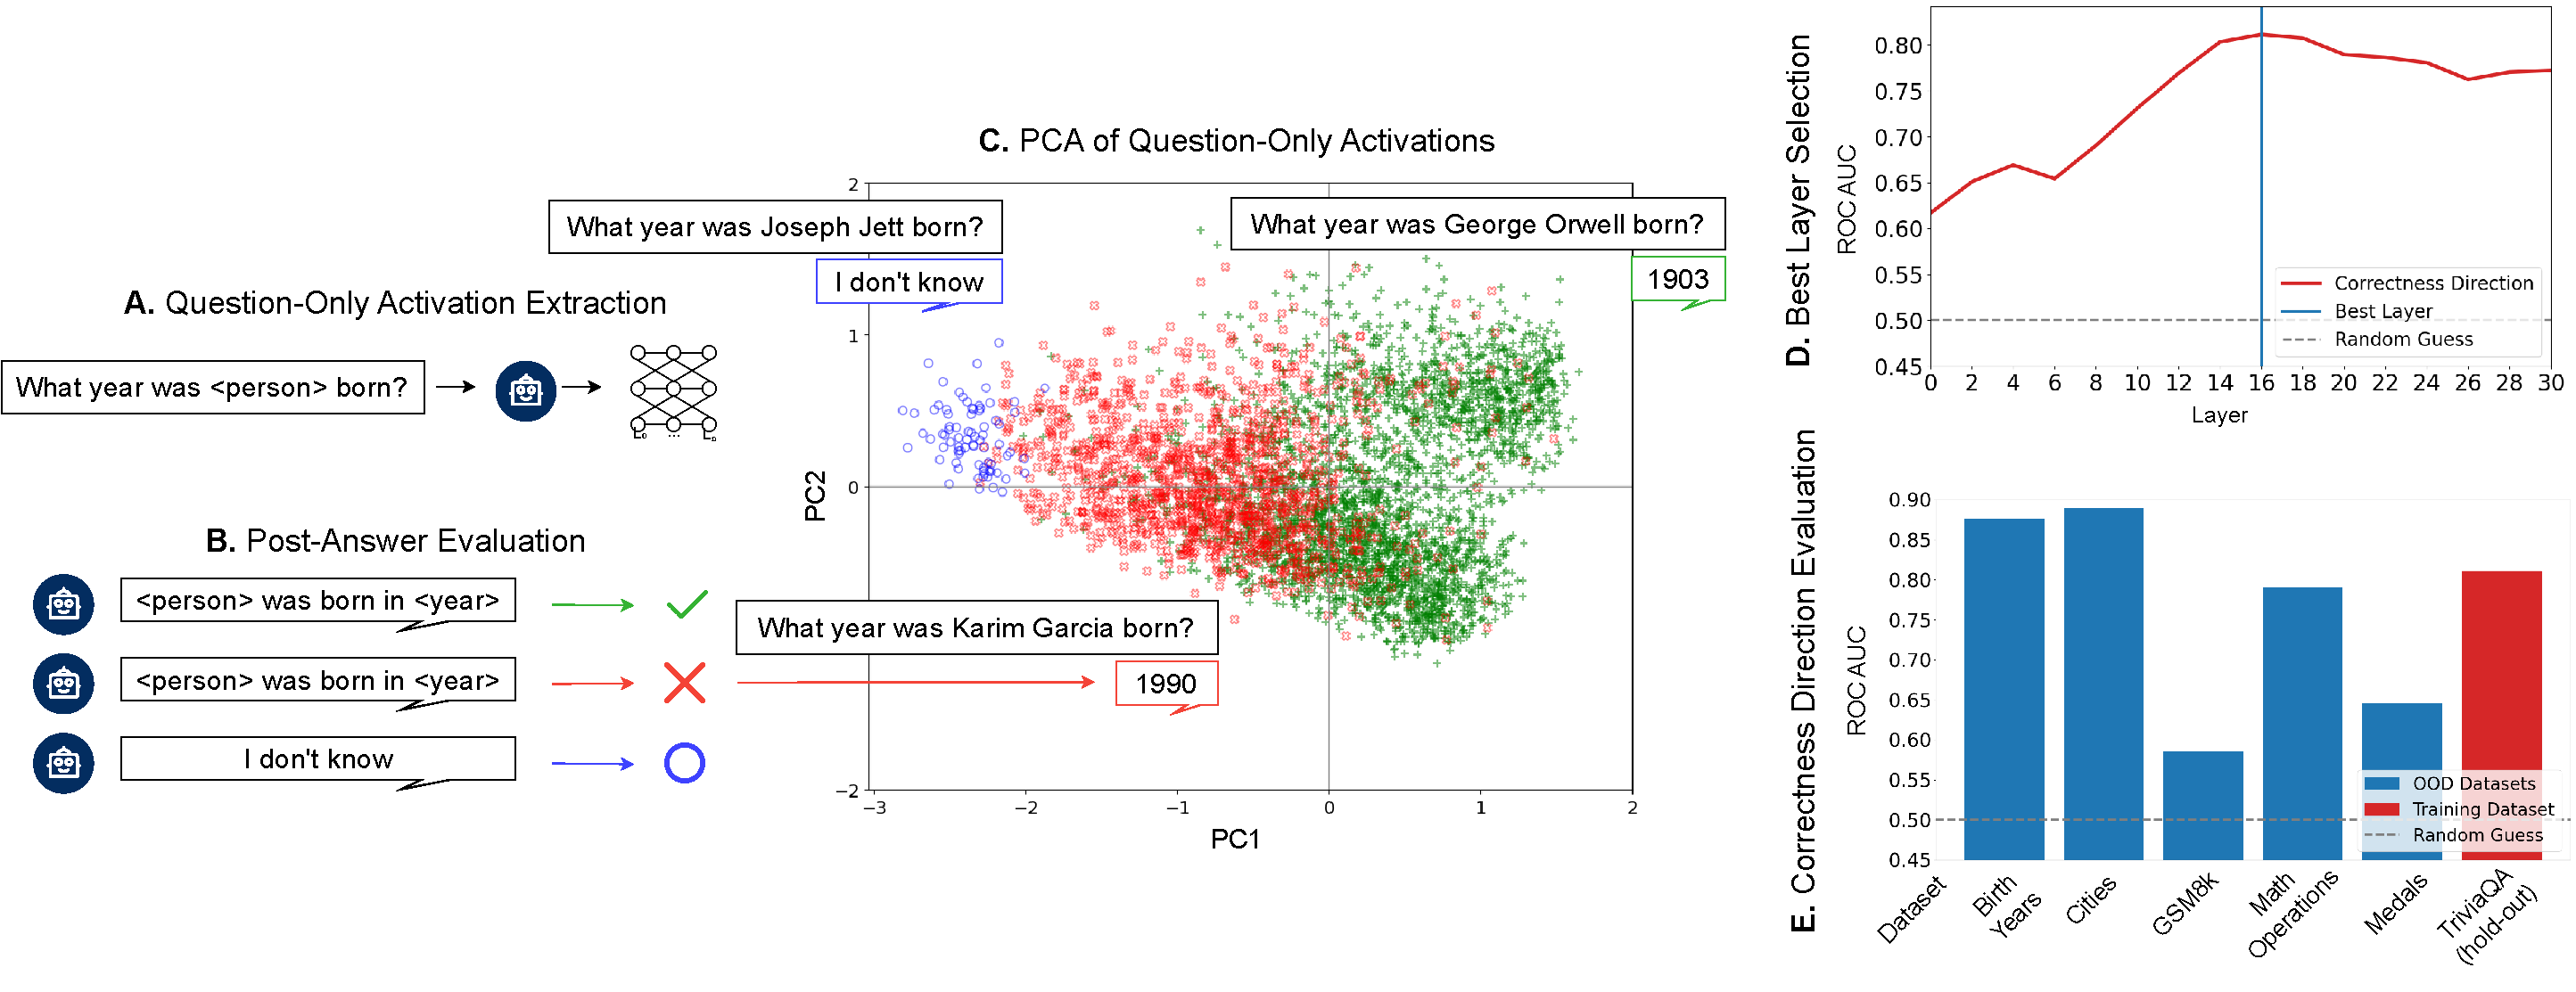
\includegraphics[width=0.88\linewidth]{diagram.pdf}
\end{center}

\small The score is defined from question-only activations before answer generation, then reused across held-out questions and datasets. Assessor averages are lower at 0.594 overall \OOD{} and 0.651 factual \OOD{}.

\vspace{0.45em}
\resultcallout{Sample efficiency is unusually high: about 160 questions already help, and roughly 2,560 recover the full 48,540-question training-set performance.}
}

\headerbox{Conclusions}{name=conclusions,column=3,row=0,span=1,above=footer}{
\begin{itemize}
\item These results validate the \textbf{Linear Representation Hypothesis} for factual correctness: a one-dimensional pre-answer direction already separates future right from wrong answers.
\item The linear probe outperforms black-box assessors under factual domain shift, even though the best assessor remains slightly stronger in distribution.
\item The signal emerges only after mid-layer processing, saturates later in the stack, and becomes cleaner in larger models.
\item Unprompted ``I don't know'' responses occupy the negative extreme of the same direction, indicating a latent confidence or knowledge-awareness axis.
\item Manual inspection suggests the scores are meaningfully calibrated: high-score mistakes are often near misses rather than arbitrary failures.
\end{itemize}

\vspace{0.35em}
For factual QA, the direction behaves like both a self-correctness signal and a self-awareness signal.
}

\end{poster}
\end{document}
